\section{Evidence from public SOFR settlements}\label{sec:market}\label{sec:empirical}
The empirical exercise asks whether an available option panel supports the meeting-risk allocations that a calibration would report. It separates three questions: which variances the contract calendar can distinguish, whether a specified pricing approximation fits, and which allocations remain possible when it does. The principal findings are that the full meeting vector is never identified by the selected variance panel, that fitting one strike can conceal sizeable errors at other strikes, and that a positive lower bound on a meeting variance can disappear when the background is made more flexible.

\subsection{Data and a fixed selection rule}
The starting panel contains 20,498 matched call--put strike pairs on 78 trading dates from 30 March through 14 September 2026. Each pair has numerical settlements for both sides and its underlying SR3 future from same-date \emph{final} CME Daily Bulletins. The archive is irregular: it is not a complete daily record. Matching uses the trading date printed inside each PDF, rather than the archive capture date. Cabinet quotes and blank settlements are retained in the source extraction but excluded from the matched panel. All 3,793 comparisons of extracted standard-option volume and open interest with printed contract totals agree. Missing archive captures, missing paired final sections, and the need for numerical settlements determine date availability before the calibration screen. Ten of the 78 retained dates lie within three calendar days of an FOMC decision, compared with 16 of the 121 weekdays in the sample span (before exchange-holiday exclusions). This simple comparison shows no obvious concentration around meetings, but cannot establish that archive availability is independent of market conditions.

Eris's public files supply a dated SOFR discount curve for every standard-panel date. We use exact daily factors at option expiry and both ends of the underlying reference quarter, with no interpolation or substitution of a neighbouring date. These are provider-constructed curves, not executable overnight-indexed-swap (OIS) quotes. A Federal Open Market Committee (FOMC) calendar captured on 30 March 2026 at 08:30 UTC supplies the 2026--27 meeting schedule available at the start of the sample. Its sixteen decision dates agree with the September calendar; future dates were tentative.\footnote{Public data sources: CME Daily Bulletins, \url{https://www.cmegroup.com/market-data/daily-bulletin.html}; Eris public files, \url{https://files.erisfutures.com/ftp/}; and the Federal Reserve meeting calendar, \url{https://www.federalreserve.gov/monetarypolicy/fomccalendars.htm}. The accompanying data directory preserves the source files, exact archive URLs, retrieval records, and SHA-256 hashes.}

The analysis applies the same retrospective selection rule on every date. The rule is fixed across this sample, rather than optimized separately to improve each date's fit. Retain standard options with 7--365 calendar days to expiry, expiry before accrual begins, and strikes within 25 rate basis points of the underlying futures index. An option \emph{chain} means one expiry on one underlying future. Retain a chain only if it has at least three matched strikes, including strikes on both sides of the future. This leaves \textbf{555 chains and 4,100 selected strike observations on all 78 dates}, with six to eight expiries per date. Throughout this application premiums are in rate bp, variances in bp$^2$, and background variance rates in bp$^2$ per year. Matrix exposures use ACT/360 year fractions. Counts are contract-date observations, so a contract appearing on several dates is counted several times. At each strike use the out-of-the-money option: a put when the futures index is at or above the strike, and a call otherwise. The other side remains available in the data but is not imposed through European put--call parity.

Standard and serial option months are mapped to quarterly futures under \citet{cme2026sr3options,cme2026sr3futures}. The mapping uses the contract's reference quarter, not a monthly future with the same month label. Strike code 9562, for example, is 95.625. The quoted futures index is 100 minus the futures rate in percent: an index of 95 corresponds to a 5\% rate. One index point is therefore 100 rate basis points. The separate midcurve extension contains 3,139 matched monthly strike pairs on seventeen dates; discount curves cover 2,755 pairs on fifteen dates. Only those pairs enter the midcurve analysis. The product labels S0, S2, and S3 denote options whose underlying reference quarters are respectively one, two, and three years beyond the standard option's quarter. Weekly quotes are excluded because their precise expiry-week mapping has not been verified.

\subsection{Pricing experiment and error measure}
The empirical prices are evaluated with a \emph{discounted European normal diagnostic}. This choice permits transparent inversion and exact linear optimization of the resulting variance intervals. It fixes the futures mean, uses a normal terminal index, and omits early exercise. Its purpose is to test what a transparent variance-based calibration can support before adding smile and exercise modelling. Failure can arise from the normal distribution, the fixed-mean assumption, the exercise convention, or the variance schedule. The decomposition below separates within-chain pricing error from additional restrictions across expiry chains; it does not separate distribution, mean, and exercise effects within a chain.

Let $x$ be the absolute futures-index--strike difference in rate basis points, $D$ the discount factor to expiry, and $\cV_{\mathrm N}$ the terminal variance of the normal futures-index diagnostic in squared rate basis points. Its selected out-of-the-money premium, also in rate bp, is
\begin{equation}\label{eq:normalproxy}
c_{\mathrm N}(\cV_{\mathrm N};x,D)
=D\left[\sqrt{\cV_{\mathrm N}}\,\varphi\!\left(\frac{x}{\sqrt{\cV_{\mathrm N}}}\right)
          -x\Phi\!\left(-\frac{x}{\sqrt{\cV_{\mathrm N}}}\right)\right],
\qquad c_{\mathrm N}(0;x,D)=0.
\end{equation}
It increases with $\cV_{\mathrm N}$. Each settlement interval therefore gives a variance interval by scalar inversion. For a chain, intersect those intervals across the selected strikes. A single $\cV_{\mathrm N}$ must satisfy every strike in the chain. We impose the additive schedule $\boldsymbol{\cV}_{\mathrm N}=\mathsf A\theta_{\mathrm N}$, with the same calendar matrix as \eqref{eq:panel} and nonnegative meeting and background variance parameters $\theta_{\mathrm N}$. The baseline meeting-risk ranges refer to these diagnostic parameters.

This distinction in notation matters. In the exact cash model, for $S<a$, the forward-measure variance of the futures rate in decimal units is
\[
\Var^{S}(F_S)=\frac{m^2}{\delta^2}\left(e^{\delta^2\cV(S)}-1\right),
\]
where $\Var^{S}$ denotes variance under the expiry-forward measure used in Proposition~\ref{prop:pricing}. It is approximately $m^2\cV(S)$ for small log variance, rather than exactly $\cV(S)$. The normal diagnostic fixes a different mean and omits this nonlinear transformation as well as early exercise. Its rejection is consequently not a rejection of the exact theoretical model, and its fitted meeting variances are not exact estimates of that model's $v_i$.

We consider three background specifications. The first has one constant variance rate. The second has separate rates on successive 90-calendar-day cells measured from the valuation date, truncating the last cell at the last expiry. The third has a separate rate in every observed expiry gap. In each case rates and meeting variances are nonnegative. The 90-day and expiry-gap grids are different partitions; neither flexible specification is asserted to contain the other.

For each date and specification, the \emph{minimum price tolerance} is the smallest common absolute premium error that permits a feasible allocation. We compute it by bisection in premium units and linear feasibility in variance units, to 0.0001 bp. A minimum tolerance of 1.5 bp means that even the best allocation has an absolute pricing error of at least 1.5 bp at some selected strike. The fixed scenarios $\pm0.25$, $\pm0.5$, and $\pm1$ bp are sensitivity choices, not historical bid--ask spreads or confidence levels.

The archived rulebook specifies a settlement increment of 0.0025 index points, or 0.25 premium bp, for all options \citep[Rule 460A01.C]{cme2026sr3options}. Outright trade increments are generally 0.5 bp, reduced to 0.25 bp for specified nearby contracts and low-premium cases (the stated premium threshold is 0.05 index points, or 5 bp). Thus the tolerances span one, two, and four settlement increments. Rounding to the nearest settlement increment alone would give at most 0.125 bp error relative to an unrounded settlement value. It would not bound disagreement with an executable price or a model value.

Discounting is material at these scales. Keeping the inferred variance fixed, removing discounting changes the nearest-strike premium by a median 0.165 bp and a maximum 1.781 bp across the 555 chains. Discounting is therefore included in all reported empirical calculations.

\subsection{The calendar and the price fit give different answers}
No date has full column rank for all meetings and the constant background rate over the selected horizon. The calendar contains six to nine meetings against six to eight expiries. On 53 of the 78 dates, the number of meetings alone is at least the number of expiries, so estimating an additional background rate already fails the dimension count. On the remaining dates, the arrangement of meeting-free gaps and meeting-containing gaps fails the calendar criterion. Individual meetings can nevertheless be identified as linear quantities. The median number individually identified is four with constant background, three with 90-day cells, and zero with a separate background rate in every expiry gap. These are interior rank statements for the design matrix $\mathsf A$ applied to the empirical parameters $\theta_{\mathrm N}$, not estimates of the exact model\'s log-variance parameters. At a boundary, nonnegativity can determine a coordinate despite deficient rank; the endpoint optimizations below detect this when its lower and upper bounds coincide. A zero lower bound alone means only that zero remains feasible.

On 11 September the individually identified count falls to zero because the January 2027 chain is absent from the selected panel. Its meeting-free gap after the December expiry had identified constant background; without that gap the background can trade against every observed meeting group. The January chain returns on 14 September and the count recovers to five. Thus the dip reflects contract selection as well as the changing horizon.

\begin{figure}[ht]
\centering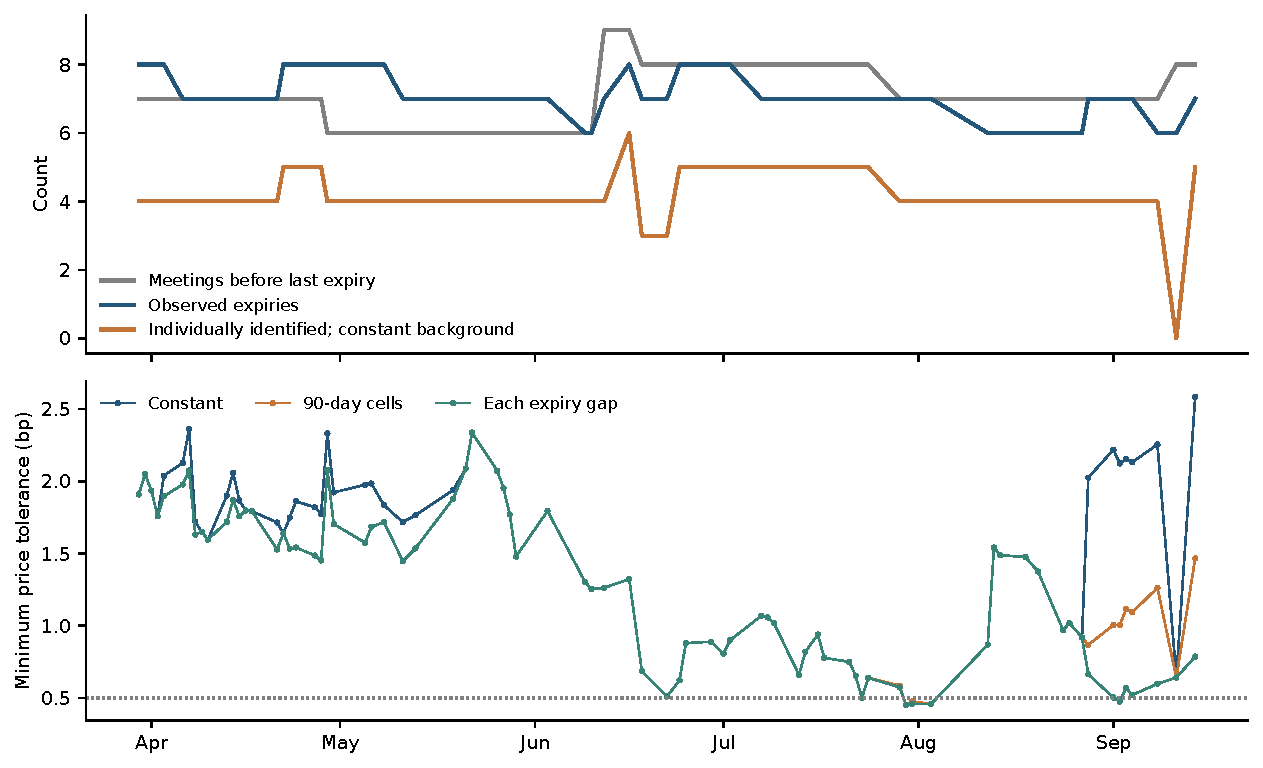
\includegraphics[width=.96\textwidth]{figures/empirical_calendar_fit.pdf}
\caption{Calendar information and price compatibility across the 78 observed dates. Top: numbers of meetings, expiries, and individually identified meeting variances under constant background. Bottom: the minimum premium tolerance needed to fit all selected out-of-the-money strikes under the discounted normal diagnostic. The dotted line is 0.5 bp. Lines connect the irregular observations; the contract set changes as expiries roll.}\label{fig:empiricalcalendar}
\end{figure}

Table~\ref{tab:empiricalfit} shows that calendar flexibility alone does not resolve the pricing problem. With constant background, only four dates fit at 0.5 bp and 23 fit at 1 bp. Even with a separate background rate in every expiry gap, only five dates fit at 0.5 bp. No specification fits any date at 0.25 bp. These are deterministic compatibility counts for this sample, not a statistical rejection frequency for the market population.

\begin{table}[ht]
\centering\small\begin{tabular}{lrrrr}\toprule Background variance & Median min. error & $\pm0.25$ & $\pm0.5$ & $\pm1$ \\\midrule
Constant & 1.683 & 0 & 4 & 23 \\
90-day cells & 1.449 & 0 & 4 & 24 \\
Each expiry gap & 1.411 & 0 & 5 & 30 \\
\bottomrule\end{tabular}

\caption{Minimum-error diagnostics and numbers of feasible dates out of 78. The second column is the median minimum tolerance, in premium bp; the remaining columns count dates fitting all selected strikes within the stated tolerance.}\label{tab:empiricalfit}
\end{table}

Using just the closest strike at each expiry makes the fit look substantially better. The median minimum tolerance falls from 1.683 to 0.247 bp for constant background. With an expiry-gap background, every date's closest-strike panel fits to within the numerical tolerance of 0.0001 bp. This is a weak fit test: any nondecreasing cumulative variance sequence can be reproduced with zero meeting variances by assigning each increment entirely to its gap's background rate. Yet the median minimum tolerance using all selected strikes remains 1.411 bp. A flexible variance schedule can reproduce these few inputs while missing the shape of the option prices.

\paragraph{Decomposing the fitting error.}
For each date, first allow each chain its own unrestricted normal variance and take the maximum of its chainwise minimum uniform errors. This is the smallest error possible before imposing any relation across expiries. Its median across dates is 1.411 bp, and it permits five dates at 0.5 bp and thirty at 1 bp. On all 78 dates, adding the expiry-gap model changes this benchmark by less than 0.000051 bp, below the bisection precision. The failure of that flexible specification is therefore already explained by within-chain pricing error. The calendar restrictions add no measurable minimum-error increment in this sample.

The standard sample has one retained chain per expiry on each date. Thus any additional cross-chain constraint combines expiry ordering with changing underlying quarters; these data cannot separate the two effects. The same-expiry midcurve experiment below tests the common-variance restriction across underlying quarters directly. Relative to the expiry-gap fit, constant background increases the required tolerance on 30 dates and 90-day background on nine dates, using 0.0002 bp to separate increases from numerical error. The largest constant-background increment is 1.799 bp. These additional errors arise from the variance specification, rather than additional smile error.

This conclusion is not driven solely by rows with no reported activity. As a separate screen, retain selected option sides with positive reported volume and open interest of at least 100. Each retained chain must still have at least three strikes in total, including strikes on both sides of the future. All 78 dates still have at least two chains. The median minimum tolerance with constant background is 1.410 bp. Reported activity is not a guarantee of executable liquidity, but this screen shows that the baseline discrepancy survives a simple activity restriction.

The baseline meeting-risk ranges and omitted-expiry checks are reported in Appendix~\ref{app:baseline}. The central sensitivity survives the better smile fit below: a positive meeting-risk lower bound can disappear when background variance is made more flexible.

\subsection{Same-expiry options on later futures}
Midcurves provide a different check. Under the parallel normal diagnostic, options with the same expiry have the same cumulative rate variance even when their underlying reference quarters differ. Apply the standard chain's closest-strike normal variance to a same-expiry midcurve, retaining the midcurve's own futures price, strike, and discount factor. The same chain-selection rule yields 165 comparisons on fourteen overlapping dates. The median absolute premium error is 3.438 bp and the maximum is 8.762 bp. The median midcurve-to-standard implied-standard-deviation ratios are 1.387 for S0, 1.221 for S2, and 1.225 for S3, based on 70, 58, and 37 comparisons respectively.



Ratios above one require larger terminal variance on the later windows under this diagnostic. The exponentially decaying loading in Section~\ref{sec:shape} predicts the opposite ordering for shifted equal-length windows: its averaged Brownian loading decreases with the window's start, while meeting loadings stay parallel. An increasing segment of a maturity-volatility curve, possibly followed by a hump, is therefore a relevant alternative; these ratios alone neither identify its shape nor distinguish it from smile and exercise effects. Section~\ref{sec:humpfit} fits such a shape, recomputes the exposures, and tests a withheld product.

The midcurve discrepancies are economically larger in premium units than many of the tolerance scenarios used to allocate meeting risk. They motivate testing maturity-dependent loadings and the listed exercise convention before using the parallel fit for relative value. They do not by themselves establish that midcurves are overpriced: the transported model has failed a pricing check.


\subsection{An at-the-money observation from a fitted smile}\label{sec:smileextension}
The within-chain errors need not be inherited by the calendar fit. We now fit a smile to each chain and use its interpolated at-the-money (ATM) price as the observation. An ATM smile estimate supplies a local variance proxy without integrating unobserved tails. It uses the same 555 standard chains and strike screen as the baseline.

Write the terminal futures-index displacement, in rate bp, as a mixture
\begin{equation}\label{eq:mixture}
I_S-I_0\ \sim\ \tfrac12 N(d,s_1^2)+\tfrac12 N(-d,s_2^2).
\end{equation}
The mean is fixed at the observed future. Each component has an elementary normal call formula, and their average gives a convex European price curve. Fit $d,s_1,s_2$ by unweighted least squares to the selected out-of-the-money settlements. Appendix~\ref{app:empiricalmethod} specifies bounds, starts, and convergence checks. The mixture is a price interpolant: it is not asserted to be the terminal law of the Gaussian rate model or a joint model across expiries.

Let $\widehat c_{\rm ATM}$ be its fitted ATM price and define
\begin{equation}\label{eq:smileatm}
\widehat{\cV}_{\rm ATM}=2\pi(\widehat c_{\rm ATM}/D)^2.
\end{equation}
This is the variance giving the same ATM premium in the normal formula. It is generally different from the mixture's second moment $d^2+(s_1^2+s_2^2)/2$. We apply the calendar matrix to this ATM proxy; its additivity is assessed in Section~\ref{sec:additivity}. For a sensitivity allowance $\varepsilon$ around the fitted ATM price, its interval is
\[
2\pi\{(\widehat c_{\rm ATM}-\varepsilon)^+/D\}^2
\ \leq\ \cV_{\rm ATM}\ \leq\
2\pi\{(\widehat c_{\rm ATM}+\varepsilon)/D\}^2.
\]
Write $\theta_{\rm ATM}$ for the nonnegative meeting and background parameters in the separate working equation $\boldsymbol{\cV}_{\rm ATM}=\mathsf A\theta_{\rm ATM}$. The endpoint programs are sharp conditional on these intervals and this additive ATM-variance schedule. The common empirical assumptions and interpretation of these sensitivity intervals are collected in Appendix~\ref{app:empiricalmethod}.

The median maximum strike error falls to \textbf{0.161 bp}, compared with 0.747 bp for the best one-variance normal fit; the largest mixture error is 0.918 bp. To test interpolation rather than only fit, remove the closest strike, refit, and predict that quote. Require at least five original strikes and observations on both sides after removal. This leaves 538 standard chains. Their median absolute held-out error is \textbf{0.124 bp}, and their maximum is 1.338 bp. These results support using the fitted ATM value as a local summary while showing that a quarter-basis-point allowance is not universally adequate.

\begin{table}[ht]
\centering\small
\begin{tabular}{lrrrr}
\toprule
Background & Median minimum (bp)& $0.25$ bp & $0.5$ bp & $1$ bp\\
\midrule
Constant &0.215&43&67&71\\
90-day cells &0.006&63&69&76\\
Each expiry gap &$<0.0001$&78&78&78\\
\bottomrule
\end{tabular}
\caption{Calendar compatibility of smile-fitted ATM observations. Counts are feasible dates out of 78. Tolerances surround fitted ATM premiums, so these counts are not directly comparable to the all-strike settlement counts in Table~\ref{tab:empiricalfit}.}\label{tab:smilefit}
\end{table}

All expiry-gap ATM panels are compatible to numerical precision. Thus the flexible calendar's failure in the baseline was not evidence against the ordering of cumulative ATM risk. Constant background still requires a median 0.215 bp allowance; additional background flexibility matters even after improving smile fit.

The meeting-risk bounds still depend on the background. On 18 June, using a 0.25 bp ATM-price allowance, the September meeting has range $[882,1080]$ bp$^2$ under constant background, $[807,1364]$ with 90-day cells, and $[0,1434]$ with expiry-gap cells. The January 2027 meeting has range $[2100,2507]$ under constant background and $[0,3371]$ under either flexible specification. Section~\ref{sec:exerciseempirical} repeats this comparison with wider expiry-specific allowances for exercise and mean effects.



A full European strip would instead identify a second moment. At pivot $x_0$, static payoff integration gives
\[
\frac2D\left\{\int_{-\infty}^{x_0}P_E(K)\,\dd K+
\int_{x_0}^{\infty}C_E(K)\,\dd K\right\}
=\Var^S(I_S)+(\E^S[I_S]-x_0)^2.
\]
It is a variance only at the expiry-forward mean. The American settlements and finite strike band here do not provide that strip: omitted tails have no finite upper bound without a tail assumption. The distinction is also relevant to the longer-sample short-rate uncertainty measure of \citet{bauer2021market}.

\subsection{Fitting a maturity loading and testing another window}\label{sec:humpfit}
Use the same smile procedure for the midcurves. First consider the bounded background loading
\begin{equation}\label{eq:humpshape}
\phi(s,T)=1+\chi\kappa(T-s)e^{-\kappa(T-s)},\qquad \chi\geq0,\quad\kappa>0.
\end{equation}
Its maximum is $1+\chi/e$ at distance $1/\kappa$, and it returns to one at long maturities. Meeting loadings remain parallel. For each shape, average the loading over each contract's window and compute the background exposures in \eqref{eq:shapeD}. We fit this matrix to the ATM proxy; Appendix~\ref{app:empiricalmethod} gives the numerical procedure and its assumptions.

There are fourteen dates with standard and same-expiry midcurve observations. Fit the common shape using the 219 standard, S0, and S2 observations, with date-specific nonnegative meeting variances and one background rate. For each candidate, solve weighted nonnegative least squares in variance, with weights $1/(2\sqrt{\widehat{\cV}_{\rm ATM}})$, then select the smallest actual standard-deviation RMSE. The original grid has $\chi\in\{0,0.5,1,2,4,8\}$ and $\kappa\in\{0.25,0.5,0.75,1,1.5,2,3\}$ year$^{-1}$: 42 parameter pairs but 37 distinct shapes. It selects $(\chi,\kappa)=(4,0.75)$. Training RMSE falls from 5.406 to 1.417 bp, while the mean absolute error on the 37 unused S3 observations rises from 1.706 to 3.818 bp.

The return to one may be too restrictive: the observed S2 and S3 volatility ratios both exceed one. We therefore add a long-end level,
\begin{equation}\label{eq:levelshape}
\phi(s,T)=1+\chi_1\kappa(T-s)e^{-\kappa(T-s)}
               +\chi_2(1-e^{-\kappa(T-s)}),\qquad \chi_1,\chi_2\geq0.
\end{equation}
This loading remains positive and bounded, with limit $1+\chi_2$. The grid in Appendix~\ref{app:empiricalmethod} has 496 distinct shapes and selects $(\chi_1,\chi_2,\kappa)=(12,8,1.5)$. Selection and date-specific fitting again use only the 219 training observations. Since $\chi_2=8$ is the primary grid's upper limit, we repeat selection on a 1,081-shape grid extending both amplitudes to 64. The same shape wins. Expanding the pure-hump subgrid to 64 distinct shapes also leaves its original optimum unchanged.

\begin{table}[ht]
\centering\small
\begin{tabular}{lrr}
\toprule
Background loading & Training SD RMSE (bp) & S3 SD MAE (bp)\\
\midrule
Parallel & 5.406 & 1.706\\
Hump returning to one & 1.417 & 3.818\\
Hump with free long-end level & 1.148 & 1.131\\
\bottomrule
\end{tabular}
\caption{Same-date product prediction: 219 standard/S0/S2 training observations and 37 S3 observations on fourteen dates. All parameter choices minimize training error. The additional family was proposed after examining the original S3 failure, so its result is a diagnostic reuse of that sample.}\label{tab:loadingcomparison}
\end{table}

Allowing the long-end level reduces S3 mean absolute error to 1.131 bp (median 1.047 bp), below both earlier specifications. Thus the original negative result is partly specific to the loading family; it does not by itself reject a common maturity loading. Figure~\ref{fig:extensions} shows where the products fall on the two selected shapes. The curves are normalized at one year because the fitted background scale absorbs their absolute level. The selected loading is 0.089 of its one-year value at zero maturity distance and 0.843 at half a year. Economically, it assigns little non-meeting volatility to the nearest forwards, consistent with a front end anchored by policy meetings. This interpretation depends on separating meeting and background risk as specified. Flattening the first half-year of the loading leaves the 22 July expiry-gap matrix rank at 12 of 15, but reduces its smallest nonzero singular value relative to its largest by a factor of 5.3. Thus exact rank does not capture how strongly the steep front distinguishes background exposures. Appendix~\ref{app:finalsensitivities} gives this controlled perturbation without refitting the model.

\begin{figure}[ht]
\centering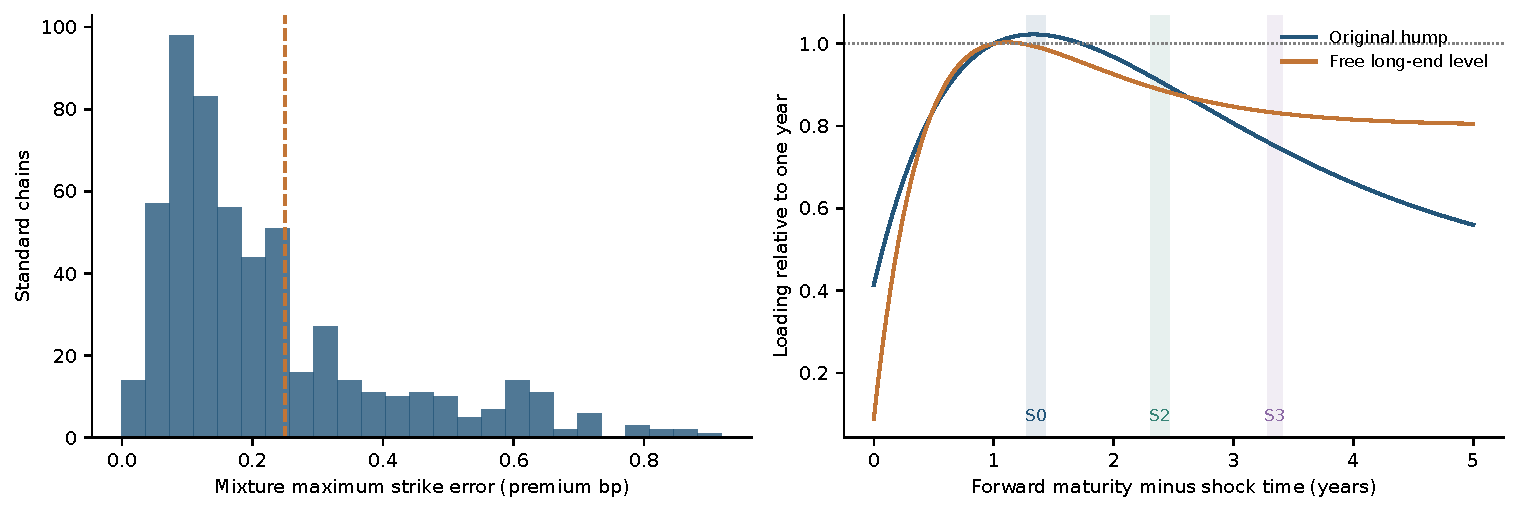
\includegraphics[width=\textwidth]{figures/empirical_extensions.pdf}
\caption{Extensions using the existing public settlements. Left: maximum selected-strike error in each standard chain's normal-mixture fit; the dashed line is 0.25 bp. Right: the two background loadings selected using standard, S0, and S2 observations, each divided by its value at one year. Shaded bands show the interquartile ranges of representative maturity distances $(a+b)/2-S/2$ for S0, S2, and S3. The exposure calculation integrates over the full accrual window and shock-time interval, not just these representative positions.}\label{fig:extensions}
\end{figure}

Each S3 exposure row lies in the span of its date's training rows, to numerical precision. Nonuniqueness of meeting allocations therefore does not alter the prediction conditional on the fitted training rows. These are point predictions, not bounds over price intervals. The new family was motivated by the earlier S3 errors; an untouched product or later sample is needed for independent validation of that family. Appendix~\ref{app:shapeprofile} retains the original-hump interval and shape-profile calculations, which show how shape uncertainty widens meeting-risk ranges.

\subsection{How large are exercise and mean adjustments?}\label{sec:exerciseempirical}
For an exercise benchmark, let the futures index be an arithmetic Brownian martingale with constant variance rate calibrated to the chain's fitted ATM variance. Discount at the constant rate reproducing its observed $D$. Value cash exercise on a recombining trinomial tree with 400, 800, and 1,600 time steps. Exercise is allowed at every step. Subtract the European value on the \emph{same} tree to isolate early exercise from terminal-payoff discretization. Appendix~\ref{app:empiricalmethod} specifies the tree and its pricing assumptions.

Use the first, middle, and last sample dates (30 March, 16 June, 14 September), and each chain's closest strike and two strike-band endpoints: 69 option observations. The 1,600-step exercise premium has median \textbf{0.023 bp} and maximum \textbf{0.377 bp}. The maximum change from 800 to 1,600 steps is 0.00050 bp; the largest European-tree error against the analytic normal price is 0.0034 bp. The largest exercise premium is for the 10 September 2027 expiry observed on 14 September 2026. Exercise is small for the median selected quote but material relative to a 0.25 bp allowance for some long expiries. It is too small in this benchmark to explain the multi-basis-point median midcurve error by itself. 

The mean effect can be sized without an exercise solver. Conditional on the 18 June ATM-proxy intervals at 1 bp, optimize the linear row $z/\delta$ in \eqref{eq:zrows}. For this sensitivity calculation only, insert those bp$^2$ allocations into the Gaussian model, converting variance to decimal units. The rate-mean displacement is
\[
F_0-\E^S[F_S]=\frac{G_0(1-e^{-z})}{\delta}.
\]
Across the three background specifications its compatible range is about $[0.00049,0.00096]$ rate bp for the first expiry and $[0.298,0.445]$ bp for the last, 11 June 2027. This is a conditional scale calculation, not a simultaneous fit of the exact cash means and variances. At fixed log variance, a European call or put price is Lipschitz in its rate mean with constant at most $D$. Hence the corresponding premium change is at most $D$ times the reported mean displacement. The longest expiries can require a wider allowance even when the smile interpolation itself is accurate.

We now widen the 18 June ATM-price allowances by both benchmark effects:
\begin{equation}\label{eq:robustallowance}
\varepsilon_\ell=0.25+\widehat{\mathrm{EEP}}_\ell
                         +D_\ell\overline{\Delta m}_\ell\quad\text{premium bp}.
\end{equation}
Here $\widehat{\mathrm{EEP}}_\ell$ is the 1,600-step exercise premium evaluated at the fitted ATM variance and zero moneyness. The mean bound $\overline{\Delta m}_\ell$ is the largest upper displacement across the three background specifications, each computed from its 1 bp seed intervals. This gives the same allowance for all three comparisons. The resulting allowances range from 0.253 to 0.989 bp across the seven expiries. Every allowance remains below 1 bp, so each new feasible set lies within the seed set used to bound its mean adjustment. The largest 800-to-1,600-step exercise change is 0.000033 bp.

\begin{table}[ht]
\centering\small
\begin{tabular}{lrr}
\toprule
Background & 16 September 2026 & 27 January 2027\\
\midrule
Constant & $[858,1100]$ & $[1910,2696]$\\
90-day cells & $[754,1384]$ & $[0,3560]$\\
Each expiry gap & $[0,1456]$ & $[0,3560]$\\
\bottomrule
\end{tabular}
\caption{18 June meeting-variance ranges in bp$^2$ with the expiry-specific allowances \eqref{eq:robustallowance}. Endpoints are rounded to the nearest bp$^2$.}\label{tab:robustranges}
\end{table}

The positive constant-background lower bounds survive (Table~\ref{tab:robustranges}). Relative to the 0.25 bp calculation, January's lower bound falls from 2,100 to 1,910 bp$^2$; allowing a flexible background still reduces it to zero. This establishes sensitivity to the background even after the specified exercise and mean allowances. The exercise estimate is a normal-model benchmark, not a uniform upper bound for every American model; the mean bound is conditional on inserting the proxy allocations into the Gaussian model.

\subsection{Does an ATM variance add across discrete meetings?}\label{sec:additivity}
A good smile interpolation does not guarantee an additive variance observation. For a centred terminal displacement $X$, the ATM proxy is $(\pi/2)(\E|X|)^2$. Independent Gaussian increments make it additive, but independent discrete increments generally do not. Consider equal-probability jumps of $\pm25$ bp. One jump and the sum of two such jumps both have $\E|X|=25$ bp, so both have ATM variance $625\pi/2=981.75$ bp$^2$, although their true variances are 625 and 1,250 bp$^2$. Adding two one-meeting ATM proxies overprices the two-meeting ATM call by 5.126 bp when the meetings are at $1/8$ and $2/8$ year and discounting is at 4\%.

Adding independent Gaussian background moderates the error but need not reduce it below 0.25 bp. With background volatility 50 bp per square-root year, eight equally spaced meetings produce a maximum ATM-price discrepancy of 2.323 bp from the additive one-increment proxy. If instead the additive schedule is allowed to fit each expiry exactly, its implied meeting variances range from 549 to 770 bp$^2$, despite all true meeting variances being 625 bp$^2$. The largest allocation errors occur at the first two meetings (770 and 549 bp$^2$); by the third, the inferred variance is 633 bp$^2$. In this example the error is concentrated where little background risk has accumulated, precisely the nearest meetings that front-end users often want to isolate. Appendix~\ref{app:additivity} gives the exact calculation and further background levels. The exercise-and-mean allowances above do not address this structural proxy error. The empirical ranges identify allocations within the additive ATM specification; interpreting them as variances of discrete policy outcomes requires a distributional pricing model or an additional sensitivity analysis.

Actual variance is additive across independent increments under a common measure, regardless of their distribution. As a companion check, Appendix~\ref{app:finalsensitivities} uses the fitted mixture second moments for the 18 June panel. This replaces the nonlinear ATM transform but introduces tail extrapolation. With the same ATM-scale perturbations and an additional 10\% moment allowance, constant-background September and January ranges are $[275,1058]$ and $[1549,4229]$ bp$^2$; both flexible backgrounds allow zero for both meetings. At 25\%, September's constant-background lower bound also vanishes and January's falls to 91 bp$^2$; at 50\%, both vanish. Without the additional allowance, constant and 90-day backgrounds are infeasible. Thus the background contrast appears under both proxies at a stated sensitivity level, but positive lower bounds are not robust to arbitrary tail uncertainty.

